% Thesis template by Aleksander M. Stensby
% aleksander.stensby@gmail.com

\documentclass[12pt,letterpaper,final]{report}
%\documentclass[12pt,a4paper,final]{report}
\usepackage{makeidx}
\usepackage{varioref}
\usepackage{setspace}
\usepackage{times} % Use this package for times-font. %%not found
\usepackage{fancyvrb}
\usepackage{moreverb}
\usepackage{fancyhdr}
\usepackage{epsfig}
\usepackage{eucal}
\usepackage{amsmath}
\usepackage{amsfonts}
\usepackage{floatflt}
\usepackage{tocbibind}
\usepackage{wrapfig}
\usepackage{listings}
\usepackage{color}
\usepackage{amsthm}
\usepackage{subfigure}
\usepackage{longtable}
\usepackage{url}
\usepackage{multicol}
\usepackage{array}
\usepackage[style=list,toc=true]{glossary}
\usepackage{graphicx} %For � kunne inkludere grafikk
\usepackage{hiafrontpage} % For UoA Style frontpage.
\usepackage{rotating}

\definecolor{Brown}{cmyk}{0,0.81,1,0.60}
\definecolor{OliveGreen}{cmyk}{0.64,0,0.95,0.40}
\definecolor{Keyword}{cmyk}{0.66,0.90,0.33,0.20}
\definecolor{Comment}{cmyk}{0.88,0.35,1.00,0.30}
\definecolor{Identifier}{cmyk}{1,1,1,1}
\definecolor{XmlKeyword}{cmyk}{0.66,0.90,0.33,0.20}
\definecolor{FrameColor}{cmyk}{0.66,0.90,0.33,0.20}
\definecolor{XmlIdentifier}{cmyk}{0,0.81,1,0.60}
\definecolor{XmlString}{cmyk}{1,1,1,1}


%%%% Fancy
% 11pt font
%\headheight=13.6 pt

% 12pt font
\headheight=14.5 pt

\pagestyle{fancy} 
\fancyhead[L]{\leftmark}
\fancyhead[R]{}
%lowercase
%\renewcommand{\chaptermark}[1]{\markboth{#1}{}}

%Fit more figures on a page
\renewcommand{\topfraction}{.99}
\renewcommand{\bottomfraction}{.99}
\renewcommand{\textfraction}{.01}
\renewcommand{\floatpagefraction}{.99}

% spacing:
%\singlespacing
\onehalfspacing
%\doublespacing

\theoremstyle{definition}
\newtheorem{theorem}{Theorem}
\hyphenation{theorem}
\newtheorem{definition}{Definition}
\newtheorem{remark}{Remark}

\oddsidemargin=0.5in \evensidemargin=0.3in
\parskip=0.0 true in

\author{Your name here}
\titlelogo{images/uia_logo_large} %Path to UoA logo.
\title{Title of your project goes here}

\draftversion{3.6}
%\date{January 9, 2007} %specify own date

\makeglossary

%for draft work, select the chapters to include in the pdf but still keep all cross-references intact.
%\includeonly{introduction}

\begin{document}

    \maketitle

    \newpage    
    \begin{abstract}
Your absctract goes here. 
Thesis template by Aleksander M. Stensby.
\end{abstract}

    \chapter*{Preface}

Your preface goes here.

    \tableofcontents
    \listoffigures
    \listoftables

    \parskip=0.1 true in

    \newpage

		% General structure, normally (background, and solution chapter may be split into several different chapters!
    \chapter{Introduction}
\label{ch:introduction}

\textit{Approx. 10 pages}

This document forms a general structure for a thesis.
Normally, background, and solution chapter may be split into several different chapters!

\section{Introduction}

\section{Motivation}

\section{Goal}
Goal of the thesis.

\subsection{Field of research}

\section{Thesis definition/objective / Statement of the Problem}

\section{Contributions}
 
\section{Target audience}


\section{Report outline / Thesis Organization}
    
    \chapter{Background}
\label{ch:background}

\section{Sample stuff}
Some simple and useful latex formatting.

\subsection{Quotations and citing}
It is explained in detail in \cite[Ch.20]{Norvig03} that 
\begin{quotation}
\noindent \textit{``the true hypothesis eventually dominates the Bayesian predication. For any fixed prior that does not rule out the true hypothesis, the posterior probability of any false hypothesis will eventually vanish, simply because the probability of generating ``uncharacteristic'' data indefinitely is vanishingly small.''}
\end{quotation}
\subsection{Figures}
This distribution, and its probability density function, is displayed in Figure \ref{fig:gaussian_distr_pdf}.
\begin{figure}[ht]
	\center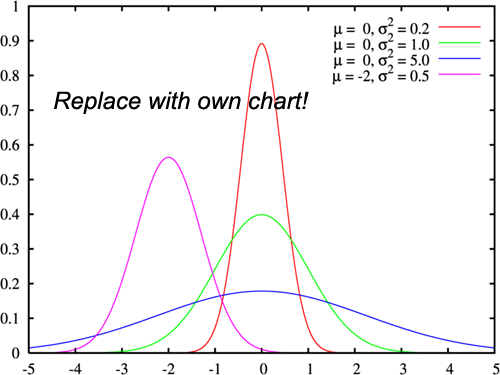
\includegraphics[width=10cm]{images/normal_distr_pdf}	
	\label{fig:gaussian_distr_pdf}
	\caption{The Normal distribution PDF.}
\end{figure}

\subsection{Equations}
By using these probabilities, and Bayes formula, we can derive the Bayes classifier.
\begin{equation}
	P(\omega_i | \boldsymbol{x}, \mathcal{X}) = \frac{p(\boldsymbol{x}|\omega_i, \mathcal(X))P(\omega_i|\mathcal{X})}{\sum_{j=1}^{c}p(\boldsymbol{x}|\omega_j, \mathcal{X})P(\omega_j|\mathcal{X})},
	\label{eq:bayes_formula_1}
\end{equation}
when we can separate the training samples by class into $c$ subsets $\mathcal{X}_1, \ldots, \mathcal{X}_c$, with the samples in $\mathcal{X}_i$ belonging to $\omega_i$.

            
    \chapter{Proposed Solution}
\label{ch:solution}
Approx. 10 pages

\section{Proposed solution / algorithm}

\subsection{The basic algorithm}

\subsection{Discussion of design issues}


\subsection{Algorithmic Enhancements}


\subsection{Discussion of the Parameter Space}


\section{Prototype}

\section{Justification of Claim to Originality}

\section{Valuation of Contribution}

\section{Alternatives}

    \chapter{Testing}
\label{ch:testing}
    \chapter{Conclusion and further work}
\label{ch:conclusion}
\textit{Approx. 5 pages}

\section{Summary of Results}

\section{Conclusion}
\emph{``My conclusion offers a compelling final comment to my argument, one that is persuasive for my
intended audience.''}

\section{Contributions}
List of contributions to new knowledge

\section{Further Work}

    \begin{singlespace}
        \bibliographystyle{IEEEtranS}
        %\bibliographystyle{plain}
				%\bibliographystyle{apalike}
        \bibliography{bib/web}
    \end{singlespace}

    \printglossary   

\end{document}

